\chapter{Kameragestützten Validierungsprozessen in der Lagerverwaltung}\label{KameragestützteInventur}

Aufgabe der Lagerzelle ist die automatische Ein- und Auslagerung von Bechern mit oder ohne Produkt.
Die Informationen die dafür übergeben werden oder entstehen müssen gespeichert werden um bei einer Produktbestellung wieder das korrekte Produkt auszugeben.
Das in \ref{Softwarearchitektur} beschriebene Datenmodell erledigt genau das. Wird ein Becher von Ort A nach Ort B bewegt, 
passieren notwendige Änderungen am Datenmodell selbst. Fehler im Datenmodell können durch systematische Tests des relevanten Quellcodes entdeckt und behoben werden. 
Zu diesem Zweck sind die Tests \verb|test\_inventory| und \verb|test_inventoryController| implementiert. 
Die Tests sind jedoch auf das Datenmodell und seinen Controller beschränkt und ein \glq ubefugter \grq Zugriff kann in Python nicht unebdingt verhindert werden. 
Eine Weitere Fehlerquelle kann die Möglichkeit der manuellen Überschreibung des Lagerbestands sein oder gar ein manueller Eingriff in der Lagerzelle selbst. 

Um diese Fehler zu erkennen soll ein kameragestütztes Inventursystem entworfen werden. 
    \section {Konzepte}
    Grundidee ist, dass eine Kamera am Greifer des Roboters so montiert ist, dass beim Abfahren existierender Wegpunkte jede mögliche Lagerstelle überwacht werden kann. 
    Mögliche Lagerorte sind:
    \begin{itemize}
        \item Der mobile Roboter in der Entladestation (Ein Becher). 
        \item Der Kommissionstisch (Zwei Abstellmöglichkeiten für Paletten)
        \item Das Lager (18 mögliche Abstellorte für Paletten)
    \end{itemize}
    Zusätzlich kann ein Becher oder eine Palette temporär von einem Greifer bewegt werden. All Diese Orte sind im Datenmodell und im GUI berücksichtigt. 
    Auf der Steuerung IRC5 des Roboters sind Routinen programmiert, die die jeweiligen Becher/Palettenbewegungen implementieren.
    Sie werden vom \verb|ABBController| aus über den entsprechenden Service via TCP aufgerufen. 

    Wenn die Kamera mittig auf dem Greifer montiert ist, kann diese Kamera erkennen ob in einem Lagerort eine Palette oder ein Becher vorhanden ist. 
    Dazu müssen an den Bechern und an den Paletten eindeutige optische Marker angebracht sein. 
    Ein entsprechendes Signal zur Bildaufzeichnung und Bildauswertung kann erfolgen, wenn der Greifer die Position vor dem Lagerort erreicht hat. 
    Da es sich bei den Produkten um eine simulierte Getränkeproduktion handelt, können sie nicht so leicht erkannt werden und sind daher nicht gegenstand dieser Arbeit. 
    
    Eine Weitere Überlegung ist, dass es keinen Mehrwert bringt Paletten voneinander zu unterscheiden, da diese nur den Zweck hat bis zu zwei Becher umfallsicher zu halten. 

    Aus der persönlichen Beobachtung der Lagerzelle reifte die Idee, dass alle Paletten und die vorderen Becher durch eine Übersichtskamera erkannt werden können. 
    Dazu wird eine Kamera mit einer höheren Auflösung in die obere Ecke der Lagerzelle gehängt. Das Regal ist dann in einem relativ kleinen Bildausschnitt im oberen Bildbereich zu sehen. 

    Der Roboter verdeckt dabei dein unteren linken Rand des Regals, sodass die Lagerpositionen L13, L14, L15 nicht erkannt werden können. 
    Die Vermutung liegt nahe, dass die Positionen L14 und L15 auch erkannt werden, wenn der Roboterarm in eine geeignete Position fährt. 
    Hier kann bspw. ein Signal der Steuerung emittiert werden, wenn der Roboterarm gerade den Becher im mobilen Roboter anfährt. 

    
    \section {Auswahl der optischen Marker}

    Die Arbeit von \cite{Hübler2019} legt die Verwendung von arUco Markern nahe. 
    Laut seiner Arbeit werden die Marker auch dann noch erkannt, wenn der vom Kamerahersteller angegebene Mindestabstand unterschritten wird und das Bild unscharf ist. 
    Der Artikel auf stackoverflow legt nahe, dass die Markerdetection robust gegenüber Rotation, Verbiegung und Knicken der Marker ist. 
    Die Marker sind quadratisch, haben einen umlaufenden Rand und eine mittige Binärmatrix. 
    Über die Binärmatrix kann auch die Orientierung des Markers ermittelt werden.
    Da jede Binärmatrix einen Integerwert darstellt, ist die Anzahl der einzigartigen ID's aus den Binärmatritzen proportional zu ihrer Kantenlänge.
    
    --> Hier Größenverhältnisse der Marker und ID Bereich beschreiben und 6x6x250 begründen.

    \section {Auswahl der Kameras, Objektive und Aufstellung}

    Die Auswahl der Kameras beruht auf meiner Semesterarbeit. Die ausgewählten Kameras sind Industriekameras und haben keine OPtik. 
    Daher erfolgt anhand des kleinsten zu erwartenden Details, des Bildbereichs sowie der Kameraparameter (Brennweite und Sensorgröße) eine Objektivauswahl. 

    Für die Übersichtskamera wurde das Objektiv auf den größtmöglichen Schärfebereich eingestellt, sodass die Chance besteht eine Markererkennung sowohl im Regal als auch im KOmmissionstisch vorzunehmen. 

    ----

    Die ursprüngliche $\mu$Eye Kamera erweist sich mit Objektiv zu lang um sie an dem Greifer zu montieren ohne die Kollisionsgefahr zu erhöhen. 
    Aus diesem Grund wird versuchsweise eine ESP32 Kamera mit verbauter Optik verwendet. Diese hat einen eingebauten Webserver, über dessen RESTful API die aufgenommenen Bilder heruntergeladen werden können. 
    Die Kamera kann von ihren Abmaßen direkt auf den Greifer montiert werden und der angegebene Mindestabstand für die Appertur wird dabei nur knapp unterschritten. 
    Testaufnahmen zeigen, dass die Marker bei gegebenen Abstandsverhältnissen noch scharf abgebildet werden. 

    \begin{figure}
        \caption[Optische Verzerrung]
        {\small bei diesem Bild wurde eine Markererkennung mit dem OpenCV Paket durchgeführt, Aus den maximalen und minimalen Koordinaten wurde ein grünes Rechteck erstellt. Aus den 4 Markern der rechten Seite und den 2 Markern links wurde der Verlauf der vertikalen Regalkanten ermittelt und das Bild so gedreht, dass die rechte Seite vertikal ist.}\label{fig:figure10}
        \includegraphics[width = \textwidth ]{Bilder/verzerrtesBild.png}
        \centering
    \end{figure}

    \section {Perspektivische Korrektur und Marker Erkennung}

    Wie in dem Bild \ref{fig:figure10} zu sehen, ist das Regal perspektivisch stark verzerrt.
    Der Verzerrung durch die Linse wird vor Allem durch die horizontale Linie deutlich, nachdem das Bild so gedreht wurde, dass der rechte Regalrand vertikal ist. 
    Für die Erkennung der Marker und der Bildsegmentierung für die Zuordnung der Marker zu den Lagerorten ist es also erforderlich entweder eine geometrische Kalibrierung der Appertur vorzunehmen oder das Bild im interessierenden Bereich zu rektifizieren. 
    Eine 4-Punkt Entzerrung ist aufgrund des geringen Aufwands und der hohen Auflösung der gewählte Weg. 
    Um die Rektifizierung zu automatisieren, wurden die oberen Regalecken und die Kreuzungen der Regalböden mit dem äußeren Rahmen mit identischen arUco Marker versehen. 
    Die obere linke Regalecke ist nicht im Bildbereich und der dortige Marker kann somit nicht erkannt werden. 
    Als die Für die 4-Punkt Entzerrung notwendigen Punkte werden die Schnittpunkte der beiden oberen Regalböden mit dem Außenrand des Regals gewählt. 
    Die eigentliche Rektifizierung ist Teil des \verb|stocktaking| Service der Software und nutzt dazu die Methoden des \verb|skimage| Pakets in Python.

    \begin{figure}
        \caption[Ablauf Bildverarbeitung und Markererkennung der Übersichtskamera]
        {\small Die ursprüngliche Aufnahme wird dupliziert. Der obere Pfad zeigt die Ermittlung der Transformationsdaten mithilfe der Regalmarker. Im Unteren PFad wird das Originalbild rektifiziert und segmentiert bevor Paletten und Becher-ID's extrahiert werden.}\label{fig:figure11}
        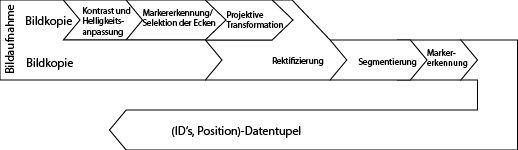
\includegraphics[width = \textwidth ]{Bilder/AblaufErkennungSellCam.png}
        \centering
    \end{figure}

    Für die perspektivische Entzerrung wird das Python Paket \verb|skimage| verwendet. Der Name steht für \glq \textbf{S}cience \textbf{K}it for \textbf{Image}processing \grq.
    Das Untermodul \verb|util.transform| enthält eine Klasse \verb|ProjectiveTransform|. Die \verb|estimate| Methode dieser Klasse akzeptiert als Parameter zwei Matritzen \verb|src| und \verb|dst| und ermittelt eine Transformationsmatrix.
    Als \verb|src| werden die Bildkoordinaten der 4 Marker angegeben und als dst die \glq realen \grq Koordinaten.
    Die \verb|warp| Methode akzeptiert neben der Instanz der o.g. Klasse auch die Eingabe- und Ausgabedimensionen. 

    Versuche haben gezeigt, dass die Erkennungsrate der Regalmarker deutlich verbessert werden kann, wenn vor der Markererkennung die Helligkeit und der Kontrast angepasst werden. 
    Noch dazu tritt eine deutliche Verbesserung der Erkennungsrate ein, wenn das Bild etwas überbelichtet ist. 
    Leider sind die Erkennungsraten der Paletten/Becher deutlich schlechter, wenn das angepasste Bild verwendet wird, welches für die Erkennung der Regalmarker optimiert ist. 
    Die Lichtverhältnisse der einzelnen Lagerplätzen sind unterschiedlich, weshalb es naheliegt den Kontrast und die Helligkeit der einzelnen Bildbereiche anzupassen. 
    Dafür wird nach der Bildaufnahme das Bild mit der \verb|copy| Funktion des \verb|numpy| Pakets dupliziert.

    Nach der Transformation des Bildes, wird das originale Bild auf die relevanten Bereiche zugeschnitten und in die jeweiligen Lagerbereiche segmentiert.
    Die einzelnen Lagerbereiche \glqq sections \grqq werden danach noch mal zwischen Palette und Becher Bereiche getrennt. 
    Danach erfolgt erneut eine Helligkeits und Kontrastanpassung bevor die einzelnen Marker in den Bildsegmenten bestimmt werden. 
    Die Bildsegmente und die erkannten Marker mit ihren ID's werden in entsprechenden Listen des \verb|stocktaking| Services gespeichert.

    \section {Automatische Kontrast und Helligkeitsanpassung}
    Wie in dem vorangegangenen Abschnitt bereits erwähnt, müssen Bilder oder einzelne Bildsegmente einer adaptiven Kontrast- und Helligkeitsanpassung unterzogen werden. 
    Dies geschieht in der Methode \verb|_automatic_brightness_and_contrast| des \verb|stocktaking| Service. 
    Die Methode bekommt als Argumente ein Bild oder Bildausschnitt als Graustufenbild, welches mit der Bildklasse des \verb|cv2| paket (OpenCV) identisch ist. 
    Außerdem wird ein Integer als ganzzahliger Prozentwert übergeben.
    Der Ablauf ist dann wie folgt: 
    \begin{itemize}
        \item Von dem übergebenen Bildausschnitt wird ein Histogramm der Graustufenskala mit einer Auflösung von 8 Bit berechnet. Dazu wird die Funktion \verb|cv2.calcHist()| verwendet.
        \item Die kumulative Verteilung des Histogramms wird berechnet.
        \item Vom unteren und oberen Rand werden so lange Werte entfernt, bis der übergebene Prozentwert überschritten ist. 
        \item Aus dem beschnittenen Histogramm werden der $\alpha$ und $\beta$ Werte für die Skalierung zu dem neuen Histogramm berechnet. 
        \item Mit den berechneten Werten für $\alpha$ und $\beta$ wird die \verb|cv2.ScaleHistAbs()| Funktion ausgeführt und so ein neues Histogramm aus den alten Werten erzeugt. 
    \end{itemize}


    \section {Markererkennung}

    Für die Erkennung der optischen arUco Marker wird aus der OpenCV Bibliothek das Modul \verb|aruco| benutzt. Die Erkennung erfolgt über die Funktion \verb|detectMarkers|.
    Auf Grundlage eines mitgegebenen arUco-Dictionarys und einem Bild oder Bildausschnitt, erfolgt eine Erkennung. 
    Der Algorhythmus und die dabei verwendeten Parameter sind in \cite{OpenCVaruco} beschrieben.
    Bei der Erkennung wird das Bild zunächst in ein binärwertiges Bild umgewandelt und anschließend nach rechteckartigen Merkmalen durchsucht. 
    Für jedes gefundene Merkmal wird die Breite des schwarzen Rahmens um die Binärmatrix ermittelt. 
    Standardmäßig entspricht die Breite des Rahmens genau einem Bit.
    Nach einer Rektifizierung wird der Bildausschnitt des Markers mit Hilfe eines Gitters in eine Binärmatrix unterteilt und decodiert. 
    Die Eckpunkte fehlerhaft decodierter oder vorangehend als nicht erkannte Marker abgelehnte Merkmale werden in der Liste \verb|rejected| ausgegeben.
    Die Ecken und ID's der erkannten Marker werden in der Liste \verb|corners| bzw. \verb|ids| ausgegeben.
    Ob die Erkennung der Marker erfogreich ist, hängt also unter Anderem davon ab das die einzelnen Bits in der Binärmatrix ähnlich breit sind. 
    
    Der Algorhytmus der Markerekennung benutzt für die einzelnen Schritte in Summe 31 Parameter, die viele Aspekte der Erkennung beeinflussen.
    Die Standardeinstellungen sind für Bilder / Bildsegmente moderater Größe eine sinnvolle Wahl. Die Erkennung versagt allerdings, wenn wie in 
    \ref{fig:figure20} der Marker durch eine Wölbung verzerrt wird, die in diesem Falle durch die 4-Punkt Verzerrung überlagert ist.
    In dem Bild ist deutlich zu erkennen, dass die Bits im rechten Bereich deutlich breiter als im linken Bereich sind. 
    Da die Marker nicht konsistent gleich angebracht sind und die Transportprozesse nicht verhindern, dass die Becher sich geringfügig drehen, ist eine Kompensation mit einem Filter 
    schwierig. 
    \begin{figure}
        \caption[Bildaufnahme aus der Lagerzelle von der Übersichtskamera.]
        {\small Die Abbildung zeigt die Aufnahme der Kamera und Appertur ohne weitere Bildverarbeitung außerhalb der Kamera. Die leichte Überbelichtung begünstigt das Erkennen der Regalmarker.}\label{fig:figure12}
        \includegraphics[width = \textwidth]{Bilder/LZIP_raw_shot.png}
        \centering
    \end{figure}

    \begin{figure}
        \caption[Bildaufnahme aus der Lagerzelle nach der Kontrastanpassung.]
        {\small Die Aufnahme aus Bild \ref{fig:figure12} nach der automatischen Helligkeits und Kontrastanpassung.}\label{fig:figure13}
        \includegraphics[width = \textwidth]{Bilder/LZ_Kontrastanpassung.png}
        \centering
    \end{figure}

    \begin{figure}
        \caption[Bild aus der Lagerzelle nach der Rektifizierung und Zuschnitt auf relevanten Regalbereich]
        {\small Die Aufnahme aus Bild \ref{fig:figure12} nach der Kontrastanpassung und Rektifizierung. Im Vordergrund sind die Paletten und Becher gut zu erkennen. Die Becher in der zweiten Reihe sind jedoch deutlich verzerrt.}\label{fig:figure14}
        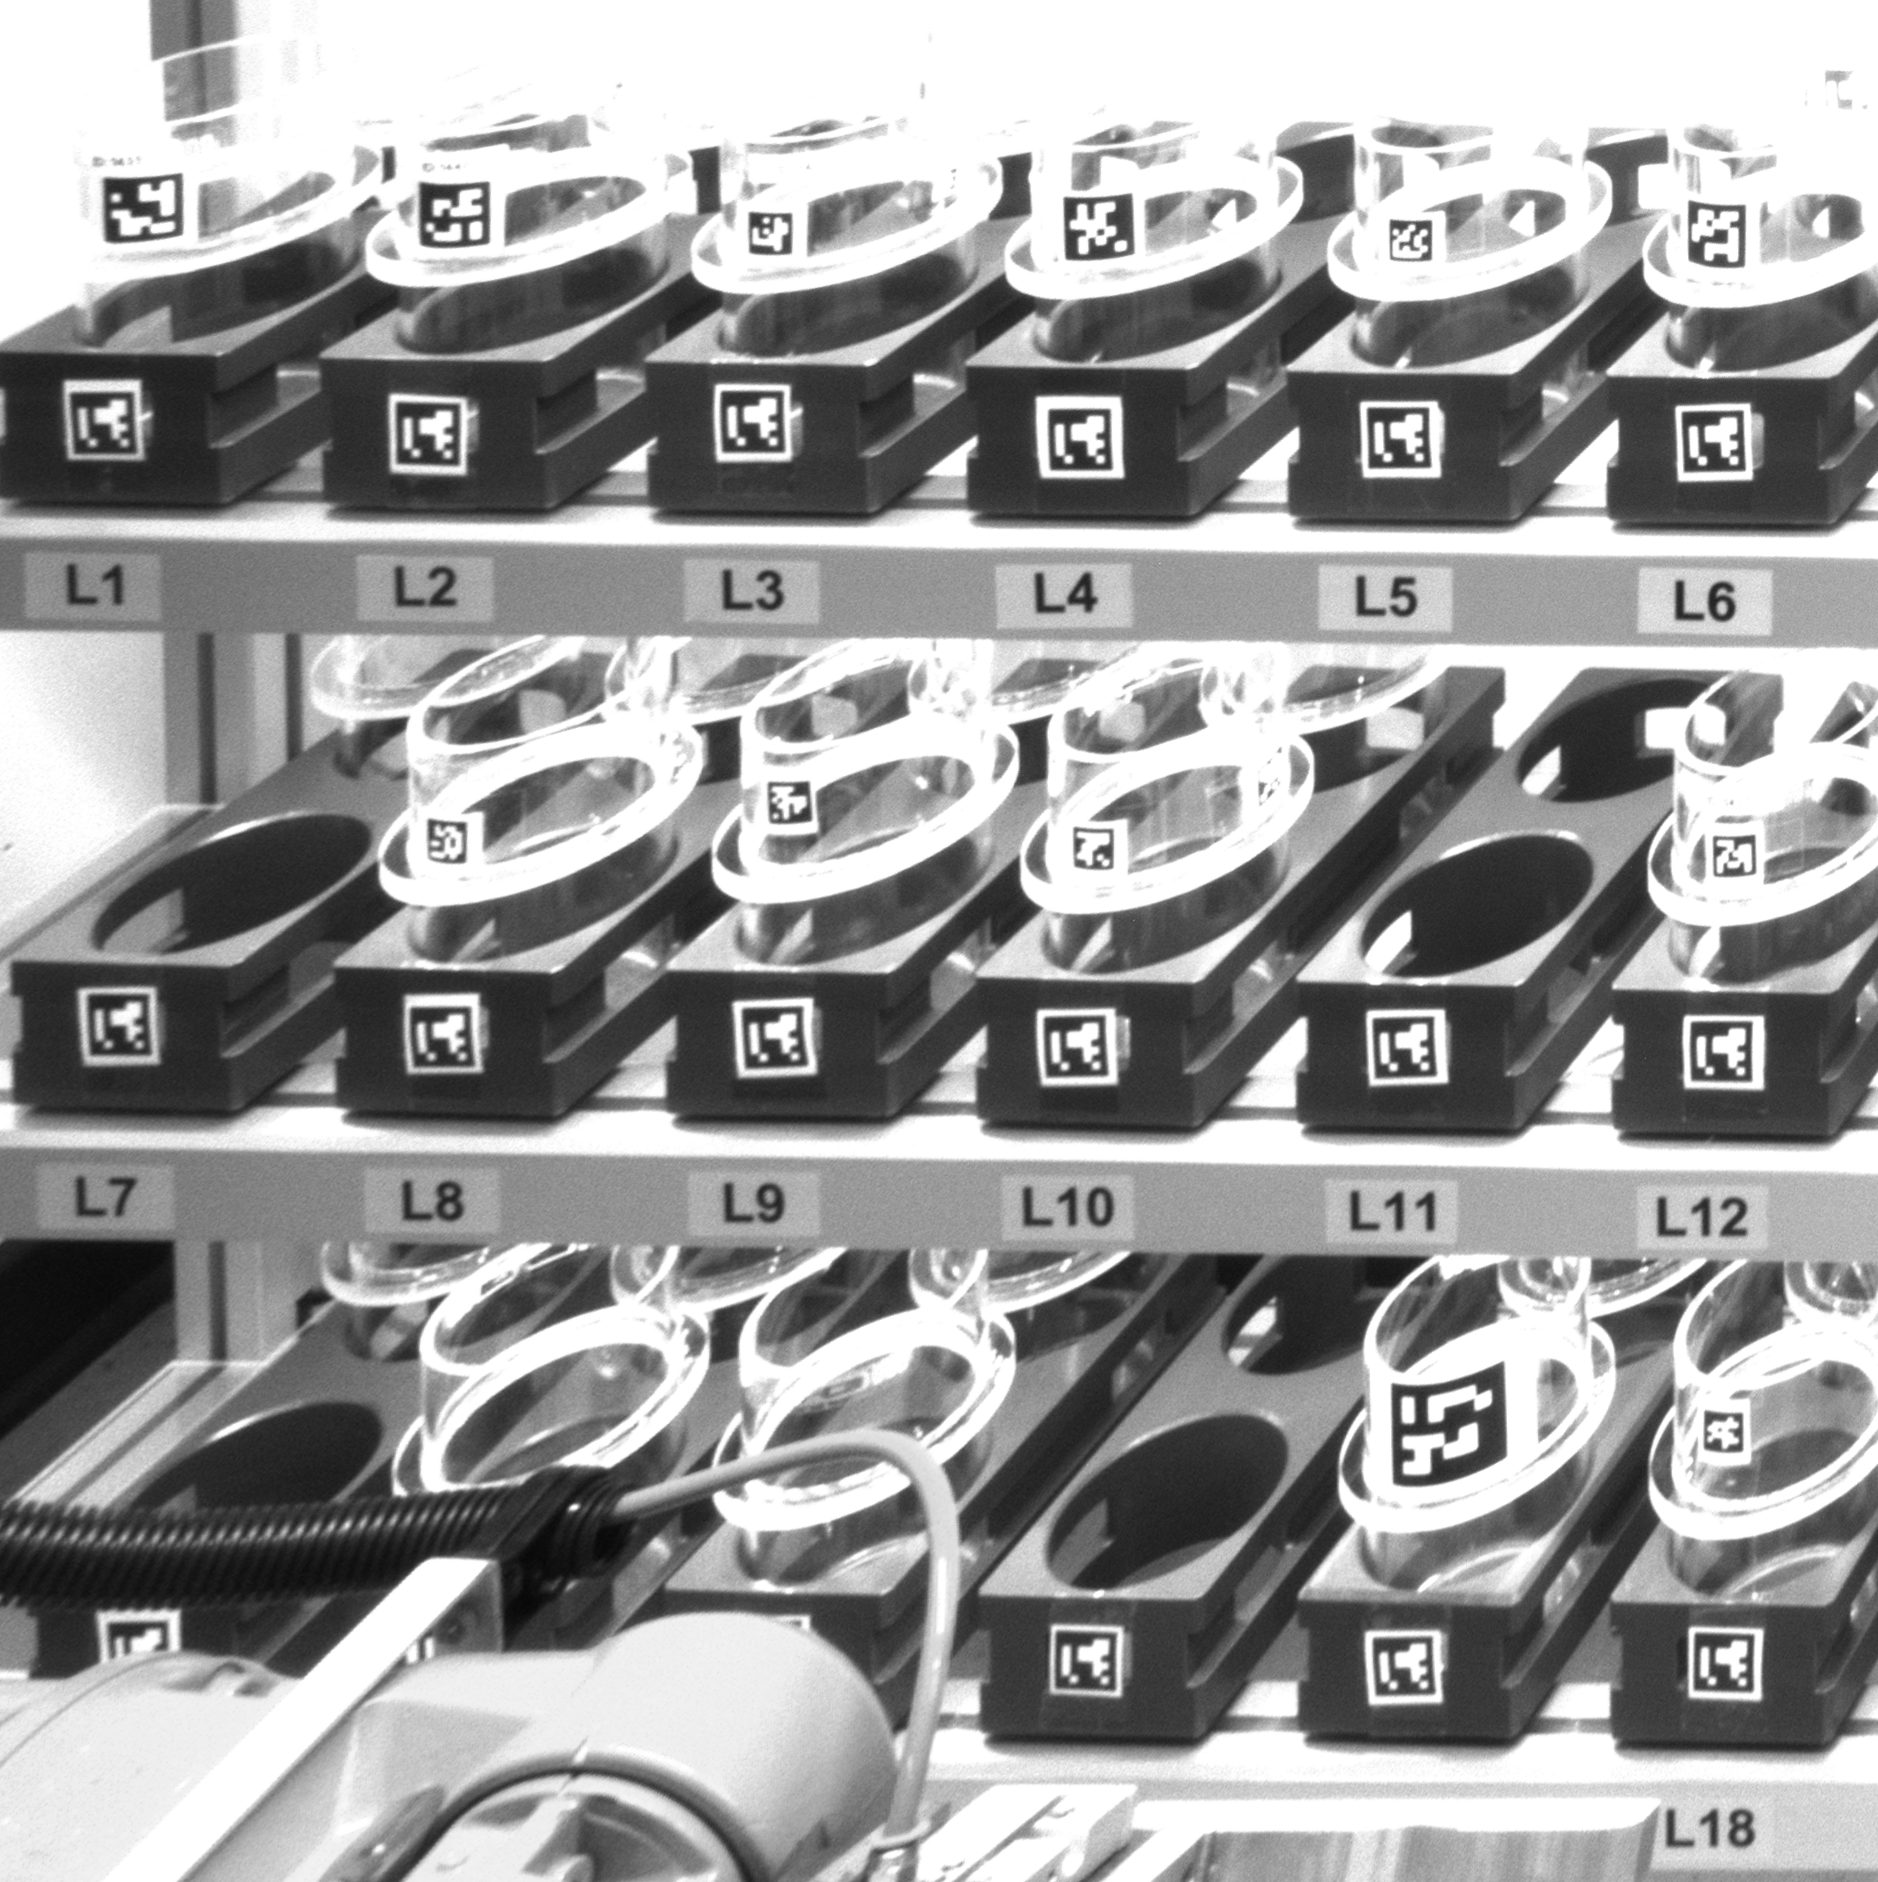
\includegraphics[width = \textwidth]{Bilder/LZ_transformed.png}
        \centering
    \end{figure}

    \begin{figure}
        \caption[Bildzuschnitt einer Lagersektion und weitere Unterteilung in die Bereiche für Becher und Palette.]
        {\small Der Bildausschnitt zeigt einen Lagerslot mit Palette aber ohne Becher im vorderen Lagerslot, der aus \ref{fig:figure15} extrahiert wurde. Der Marker hat kein weißes Rechteck um sich was bedeutet, dass dieser Marker nicht erkannt wurde. Dies liegt vermutlich an der durch die Wölbung gestörten Binärmatrix}\label{fig:figure15}
        \includegraphics*[width = \textwidth/3]{Bilder/section_16.png}
        \centering
    \end{figure}

    \begin{figure}
        \caption[Bildzuschnitt einer Lagersektion und weitere Unterteilung in die Bereiche für Becher und Palette.]
        {\small Der Bildausschnitt zeigt einen Lagerslot mit Palette und Becher im vorderen Lagerslot, der aus \ref{fig:figure15} extrahiert wurde. Der Marker hat kein weißes Rechteck um sich was bedeutet, dass dieser Marker nicht erkannt wurde}\label{fig:figure18}
        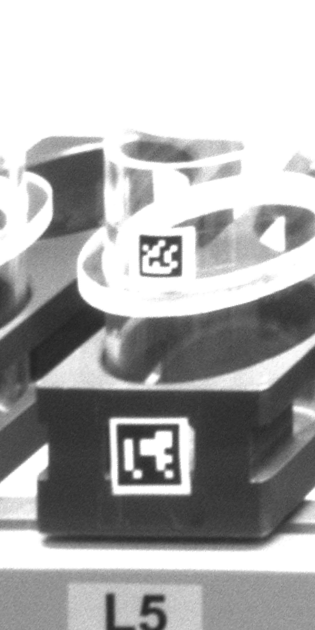
\includegraphics[width = \textwidth/3]{Bilder/section_5.png}
        \centering
    \end{figure}

    \begin{figure}
        \caption[Bild aus der Lagerzelle nach der Rektifizierung und Zuschnitt auf einen Bereich einer Palette]
        {\small Bereich einer Palette, aus \ref{fig:figure14} extrahiert. Der dicke weiße Rahmen wird im Programmcode erzeugt wenn der Marker erfolgreich erkannt wurde. }\label{fig:figure16}
        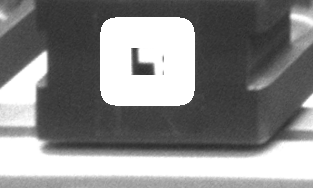
\includegraphics[width = \textwidth/3]{Bilder/pallet_5.png}
        \centering
    \end{figure}

    \begin{figure}
        \caption[Bild aus der Lagerzelle nach der Rektifizierung und Zuschnitt auf einen Bereich einer Palette]
        {\small Bereich einer Palette, aus \ref{fig:figure14} extrahiert. Im Gegensatz zu \ref{fig:figure16} wurde der Marker nicht erkannt. }\label{fig:figure19}
        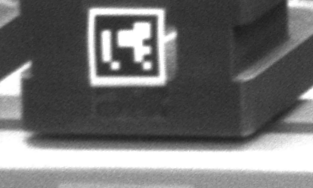
\includegraphics[width = \textwidth/3]{Bilder/pallet_3.png}
        \centering
    \end{figure}

    \begin{figure}
        \caption[Bild aus der Lagerzelle nach der Rektifizierung und Zuschnitt auf einen Bereich eines Bechers]
        {\small Bereich eines Bechers, aus \ref{fig:figure14} extrahiert. Deutlich sichtbar ist die durch die Wölbung des Bechers gestörte Binärmatrix des Markers.}\label{fig:figure17}
        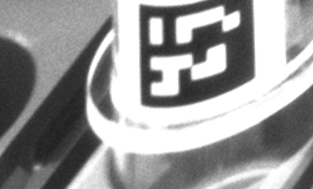
\includegraphics[width = \textwidth/3]{Bilder/cup17.png}
        \centering
    \end{figure}

    \begin{figure}
        \caption[Bild aus der Lagerzelle nach der Rektifizierung und Zuschnitt auf einen Bereich eines Bechers]
        {\small Bereich eines Bechers, aus \ref{fig:figure14} extrahiert. Auch hier ist die durch die Wölbung induzierte Verzerrung des Markers deutlich sichtbar.}\label{fig:figure20}
        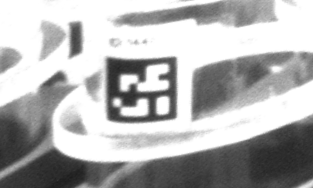
\includegraphics[width = \textwidth/3]{Bilder/cup2.png}
        \centering
    \end{figure}